\section{GMSC的仿真模拟测试}
本节使用仿真平台对GMSC的性能进行测试。具体而言,是测试GMSC能在多大程度上提升sketch测量的性能。

\subsection{测试设置}
本节中用到的测试指标为平均估计误差和最大交换机负载,
其中平均估计误差的定义与第\ref{subsec:metric}节相同。
最大交换机负载是统计每个交换机所处理的流量总和,取其最大值作为指标。
测试基准有两种,第一种是协作式CountMax,另一种是非协作式CountMax。
其中非协作式CountMax是在所有接入层交换机上都部署CountMax,每个CountMax只处理以本交换机作为出口交换机的数据包。
对于一条流被多次测量的情况,采取多个测量值的最大值作为结果。

测试拓扑采用的是与第\ref{sec:simulation}节相同的Fat-tree。
测试当中,用于计算的先验知识为所有流的准确信息和大小,掩码根据源地址与目的地址(O-D对)进行分割。
测试用的流的集合也与第\ref{sec:simulation}节相同,其中最大的一条流的大小约为9GB。
在GMSC中,每条流的价值和代价均为流的流量大小,每个交换机设置的负载上限约为10GB。

\subsection{测试结果}

\begin{figure}[ht]
	\centering
	\begin{minipage}[t]{0.48\linewidth}		
		%\begin{figure}[!t]
		\centering
		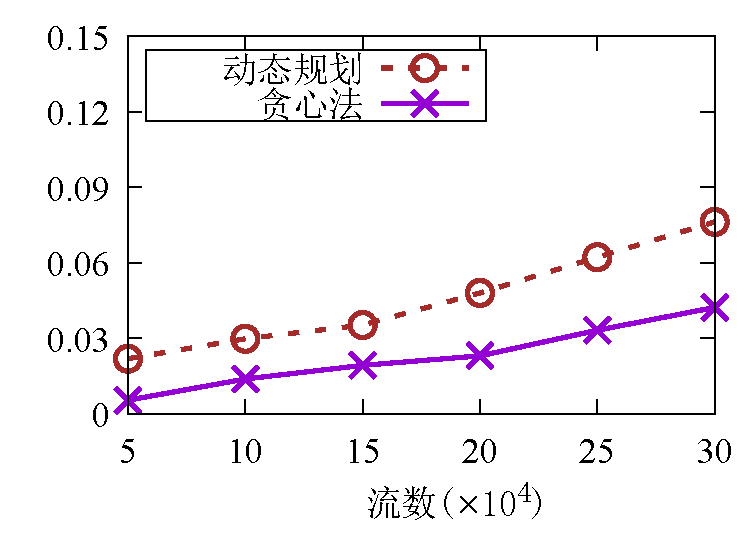
\includegraphics[width=\linewidth]{fig/msc_cmp_appr.pdf}
		\caption{\textnormal{平均估计误差与流数,$k=1000$。}}
		\label{fig:msc,appr}
		%\end{figure}
	\end{minipage}\vspace{-0.6em}\hspace{0.4em}
	\begin{minipage}[t]{0.48\linewidth}
		\centering
		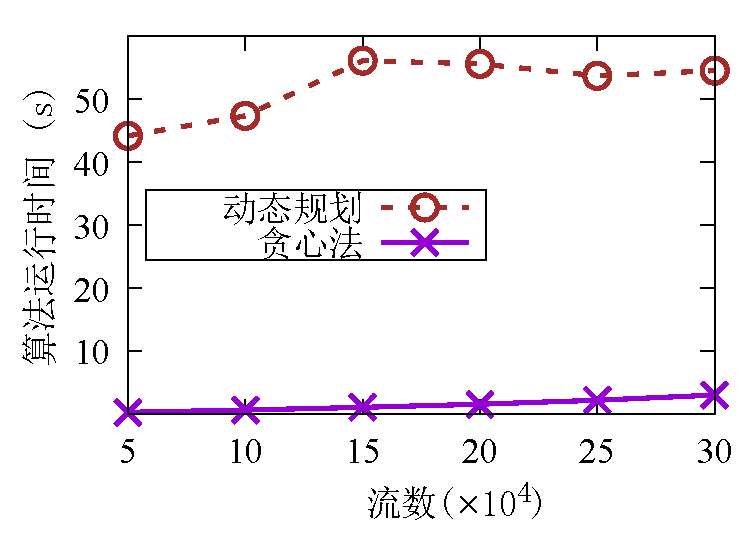
\includegraphics[width=\linewidth]{fig/msc_cmp_time.pdf}
		\caption{\textnormal{算法运行时间与流数,$k=1000$。}}
		\label{fig:msc,time}
	\end{minipage}\vspace{-0.6em}
\end{figure}

第一组测试是对比使用动态规划解背包问题的GMSC和使用贪心法解背包问题的GMSC的性能。
由于动态规划算法的时间复杂度和背包容量,即交换机负载上限呈线性关系,而测试中这一数字十分巨大,导致动态规划算法耗时极其漫长。
为了能够在合理的时间内获得结果,在这组测试中我们将流的价值和负载上限进行等比缩放(全部除以1000)后再进行动态规划。
图\ref{fig:msc,appr}中显示,由于缩放带来的误差,使用动态规划方法最终得到的估计误差反而超过了使用贪心法的误差。
图\ref{fig:msc,time}则表明,即使进行了1000倍的缩放,动态规划方法的运行时间仍是贪心法的10倍以上。
贪心法的运行时间随流数增加而增加的原因是,流数越多,每轮迭代后更新$p(\Pi_i^j)$所需的时间也会线性增加。

根据这一组实验的结果,我们决定接下来的测试中,GMSC一律使用贪心法解背包问题。

\begin{figure}[ht]
	\centering
	\begin{minipage}[t]{0.48\linewidth}		
		%\begin{figure}[!t]
		\centering
		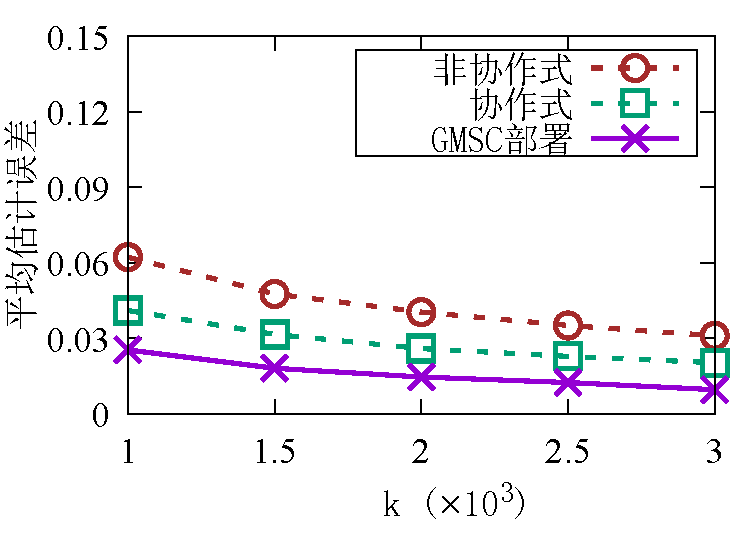
\includegraphics[width=\linewidth]{fig/msc_k_appr.pdf}
		\caption{\textnormal{平均估计误差与$k$,200000条流,$\alpha = 1\%$。}}
		\label{fig:msc,err,k}
		%\end{figure}
	\end{minipage}\vspace{-0.6em}\hspace{0.4em}
	\begin{minipage}[t]{0.48\linewidth}
		\centering
		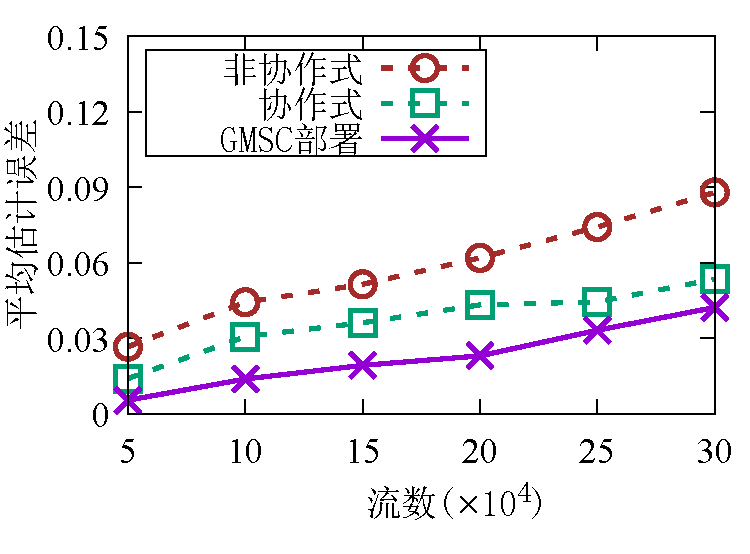
\includegraphics[width=\linewidth]{fig/msc_f_appr.pdf}
		\caption{\textnormal{平均估计误差与流数,$k=1000$,$\alpha = 1\%$。}}
		\label{fig:msc,err,flow}
	\end{minipage}\vspace{-0.6em}
\end{figure}

图\ref{fig:msc,err,k}和图\ref{fig:msc,err,flow}描述了使用GMSC部署的CountMax的估计误差与协作式和非协作式CountMax的对比。
在GMSC部署下,CountMax对网络中的大流的估计误差略有下降。和协作式CountMax相比约降低了20\%到30\%。
这主要是得益于GMSC部署将流的测量分散到各个交换机中,从而进一步减少了哈希冲突出现的概率。

\begin{figure}[ht]
	\centering
	\begin{minipage}[t]{0.48\linewidth}		
		%\begin{figure}[!t]
		\centering
		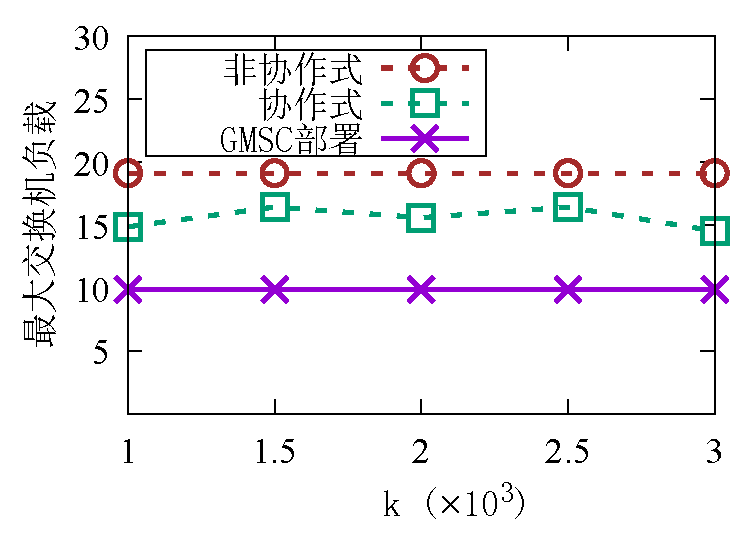
\includegraphics[width=\linewidth]{fig/msc_k_time.pdf}
		\caption{\textnormal{最大交换机负载与$k$,200000条流。}}
		\label{fig:msc,time,k}
		%\end{figure}
	\end{minipage}\vspace{-0.6em}\hspace{0.4em}
	\begin{minipage}[t]{0.48\linewidth}
		\centering
		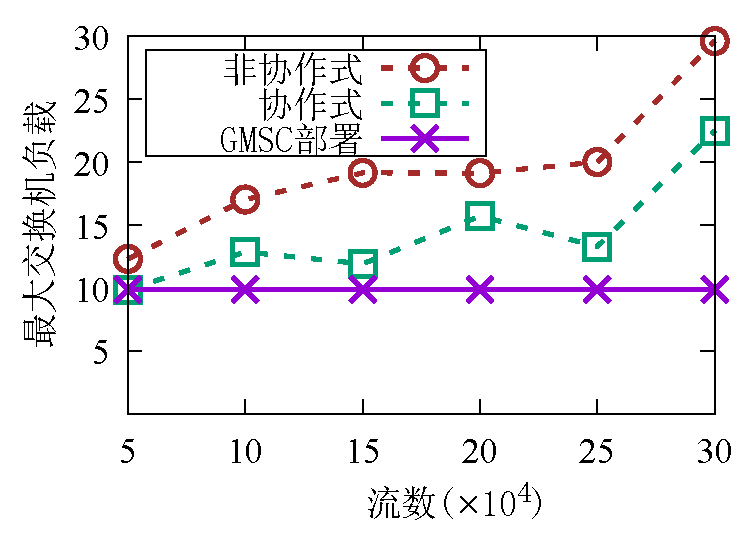
\includegraphics[width=\linewidth]{fig/msc_f_time.pdf}
		\caption{\textnormal{最大交换机负载与流数,$k=1000$。}}
		\label{fig:msc,time,flow}
	\end{minipage}\vspace{-0.6em}
\end{figure}

图\ref{fig:msc,err,k}和图\ref{fig:msc,err,flow}描述了交换机的最大负载。
由于交换机负载上限的限制,GMSC方法的最大交换机负载始终保持不变;
而协作式和非协作式的计算负载随着流数的增加明显上升,并且协作式CountMax由于引入了随机因素,导致最大交换机负载变得更加不易预测,体现在图中为较大的波动。

